\section{Introduction}
\indent Similar to the concept of the Taylor Series, 
all functions can be written as sum of cosine and sine 
functions with different weightings and frequencies. 

\vspace{25pt}
\begin{figure}[h]
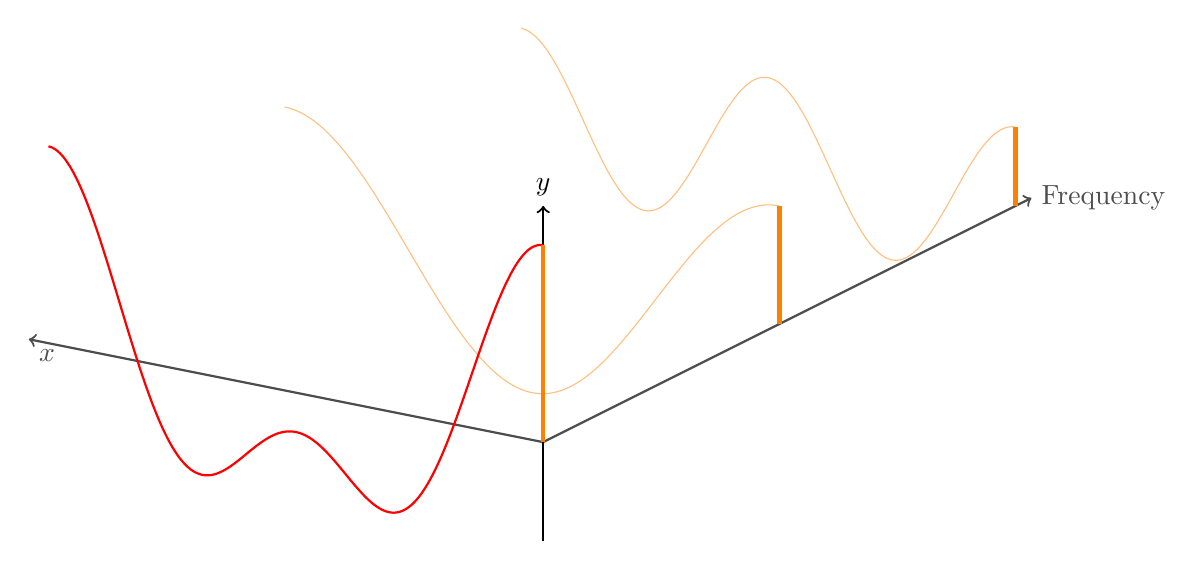
\begin{tikzpicture}[x={(1cm,0.5cm)},z={(0cm,0.5cm)},y={(1cm,-0.2cm)}]
    \draw[->,thick,black!70] (0,0,0) -- (6.2,0,0) node[right] {Frequency}; % frequency axis
    \draw[->,thick,black!70] (0,0,0) -- (0,-2*pi-0.25,0) node[below right] {$x$}; % time axis
    \draw[->,thick] (0,0,-2.5) -- (0,0,6) node[above] {$y$}; 

    \draw [orange!50, domain=-2*pi:0,samples=300,smooth] 
        plot (3,\x, {3*cos(180*\x/pi) });
    \draw[orange, ultra thick] (3,0,0) -- (3,0,3);

    \draw [orange!50, domain=-2*pi:0,samples=300,smooth] 
        plot (6,\x, {2*cos(360*\x/pi) });
    \draw[orange, ultra thick] (6,0,0) -- (6,0,2);
    
    \draw [red, thick, domain=-2*pi:0,samples=300,smooth] 
        plot (0,\x, {3*cos(180*\x/pi) + 2*cos(360*\x/pi});
    \draw[orange, ultra thick] (0,0,0) -- (0,0,5);
    
\end{tikzpicture}
\caption{an example of periodic function summation}
\label{fig:intro_example}
\end{figure}
\vspace{25pt}

\indent Figure \ref{fig:intro_example} is a periodic function, and it can be broken down into 
the sum of two cosine functions $f(x)=3\cos(x)+2\cos(2x)$.  %\newpage

This concept of transformation is the fundamental of Fourier Transform as the name suggests,
and has great application in many field of study, for example, signal processing. 
The function of time would be converted into the functions of frequency. 
It used to be difficult to isolate or manipulate some certain frequencies with the function of time, 
but we can convert/transform it into the functions of frequency, then do whatever needs to be done. 
It can be again transformed back into the function of time when needed.
